\chapter{実験}
複数タスクにかかる所要時間に対し被験者の予測とADLoggerの予測の差異を比較した上で,
ADLogger導入によって,行動・意識の変容が生じるかどうか検証を実施した.
本章ではまず実験の目的と手法を説明し,得られた実験結果のデータの概要を示す.

\section{実験目的}
本研究では,複数タスクにかかる所要時間の予測に関して被験者の予測とADLoggerの予測の差異を比較する事,
ADLogger導入によって,時間管理に対する苦手意識・行動への変化が起こる事を目的としている.

\section{実験手法}
今回の評価実験では,被験者に時間の長さを教示し,その長さを産生させる時間産生法\cite{Oguro1961}\cite{Tayama2018}を慶應義塾大学の学生男女20名に対し平日と休日(またはそれに準ずる日)にそれぞれ3回(合計6回)に渡って実施した.
始めに,被験者は事前に各自保持しているiPhoneにADLoggerをインストールして貰う.

実験は平日と休日(またはそれに準ずる日)は異なる動き・見積もりを行う可能性を鑑み,3回分の平日と休日をそれぞれ1回ずつ以上(計6回以上)実施した,
被験日はまず行動前に朝実施する日常生活動に関して行動名,行動毎の必要時間予測,タスクを連続で行った時の総合必要時間予測を申告してもらう.
尚,6回の計測を通じて予測を適宜修正できるものとする.
その後,web会議ツールであるzoom\cite{zoom}およびADLoggerを用いながら実際に行動して貰い実測値を計測する.
zoomにおいては全ての行動の開始時/終了時に連絡を行い,実験者が総合時間を計測する.
更に被験者はADLoggerを用いて行動毎の時間を計測する.
一定期間後(原則4回目)以降の計測はADLoggerのADLogおよびタイマーのカウントアップ表示を閲覧できる状態にしながら計測して貰う.
最終日にはプリケーションによる定性的効果やアプリケーションの改善点を知る為にインタビューを行う.インタビューにて質問する項目は付録Aにて記載した.

\section{実験結果}
被験者20名中,被験に協力頂いたのは19名だった.
内,被験期間内に実験を終わらせられた(被験回数6回以上,ADLogの効果比較済)のは【16】名だった.
具体的なデータ数は図~\ref{fig:day}に記載した.
\begin{figure}[hb]
	\begin{center}
	\fbox{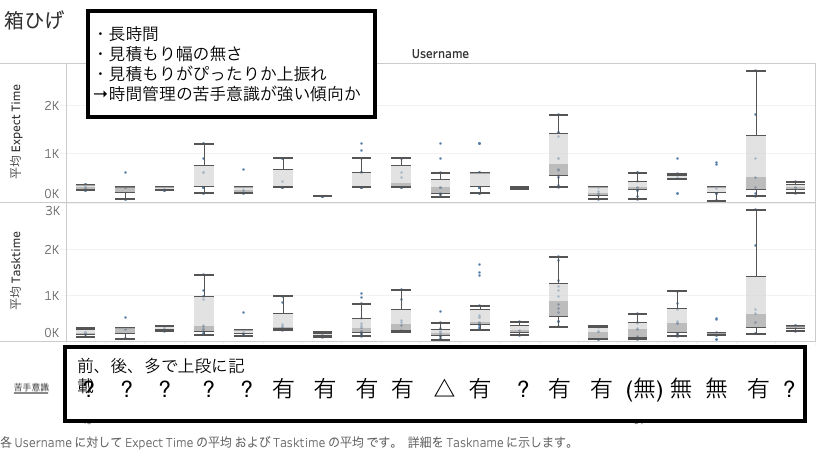
\includegraphics[width=5cm]{images/7/1.png}}
		\caption{ユーザ 別被験日数一覧}
		\label{fig:day}
	\end{center}
\end{figure}

また,被験者が行う行動・行動時間は被験者に合わせている為,行動時間には個人差がある.
図~\ref{fig:day}上部はタスク別,下部は合計時間の分布を箱髭図で描いたものであり,被験者の行動時間は個人差が大きいことが分かる.
\begin{figure}[hb]
	\begin{center}
	\fbox{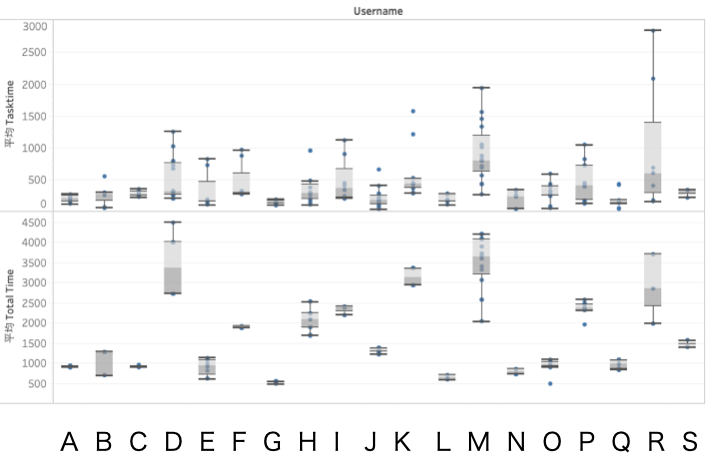
\includegraphics[width=15cm]{images/7/2.png}}
		\caption{ユーザ 別被験用時間}
		\label{fig:day}
	\end{center}
\end{figure}

さらに,ADLog導入前のタスク別予測と実測の平均時間の比較を図~\ref{fig:compare}に,総合時間の比較を図~\ref{fig:compare2}に記す.
図~\ref{fig:compare},~\ref{fig:compare2}は横軸を実測の平均時間,縦軸を予測の平均時間にしたものである.
見積もりの予測と実態に関して切片が0の一次関数で表すと,図~\ref{fig:compare}はy=【0.96】x,図~\ref{fig:compare2}はy=【0.99】xになった.
この事から被験者を全体で見ると予定の予測をぴったりかやや実測より短めに見積もる傾向がある事が分かる.
また,図~\ref{fig:compare3}は図~\ref{fig:compare}の結果を,図~\ref{fig:compare4}は図~\ref{fig:compare2}の結果をユーザ別に傾向線を引いたものである.
被験者は図~\ref{fig:compare3}は係数【1.93】から【0.69】の間で,図~\ref{fig:compare3}は係数【1.55】から【0.73】の間で見積もっていた.

\begin{figure}[hb]
	\begin{center}
	\fbox{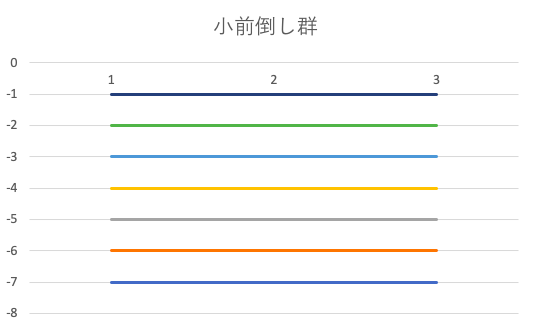
\includegraphics[width=15cm]{images/7/3.png}}
		\caption{予測と実測の平均時間比較}
		\label{fig:compare}
	\end{center}
\end{figure}

\begin{figure}[hb]
	\begin{center}
	\fbox{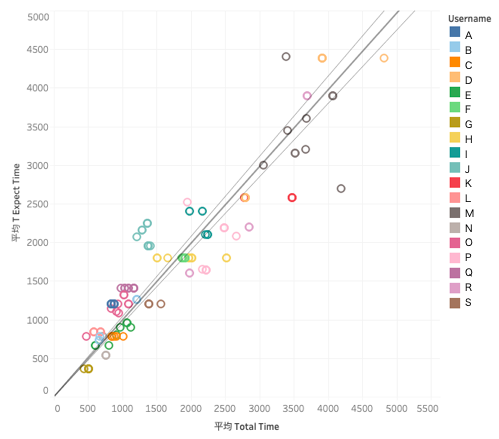
\includegraphics[width=15cm]{images/7/4.png}}
		\caption{予測と実測の平均時間比較(総合時間)}
		\label{fig:compare2}
	\end{center}
\end{figure}

\begin{figure}[hb]
	\begin{center}
	\fbox{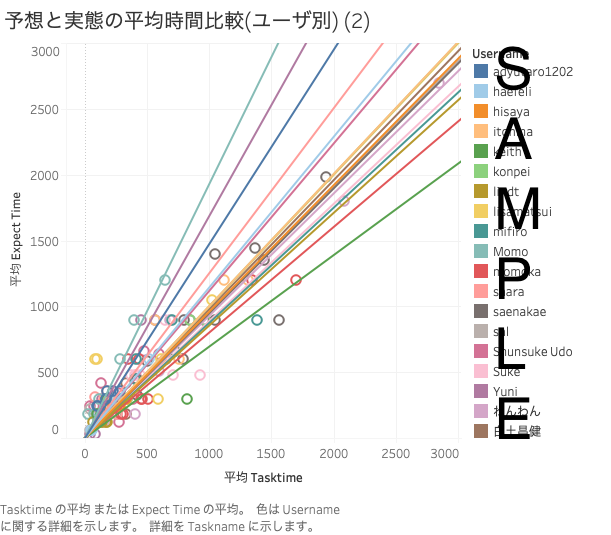
\includegraphics[width=15cm]{images/7/5.png}}
		\caption{予測と実測の平均時間比較(ユーザ別)}
		\label{fig:compare3}
	\end{center}
\end{figure}

\begin{figure}[hb]
	\begin{center}
	\fbox{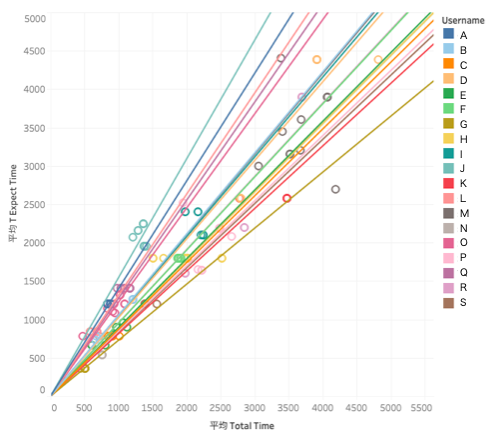
\includegraphics[width=15cm]{images/7/6.png}}
		\caption{予測と実測の平均時間比較(ユーザ別総合時間)}
		\label{fig:compare4}
	\end{center}
\end{figure}

\chapter{評価}
本研究における手法及び結果について説明する.

\section{実験評価手法}
本研究はTableau\cite{tableau}を用いて下記の通り評価を行う.
まずアプリケーションの介入によって見積もりと実測の差がどれだけ変化したか全体の比較を行う.
その後,図~\ref{fig:compare}の見積もりの係数が高い順位で並べそれぞれ変化をみた.
上位6人をグループ\UTF{2460},中位上位6人をグループ\UTF{2461},下位7人をグループ\UTF{2462}とした上で
それぞれの見積もり傾向とアプリケーションによる効果の有無を調査する.

\section{評価結果}
本節では,本システムのADLog機能導入後時間管理に対し与える影響について,本評価実験で得られた評価結果を示す.
\subsection{アプリケーションによる効果}
アプリケーションのADLog機能を導入する前と後によって係数がどう変化したかを表~\ref{fig:7}で表した.
表~\ref{fig:7}からわかる様にタスク時間,総合時間ともに係数は減少した.

\begin{figure}[hb]
	\begin{center}
	\fbox{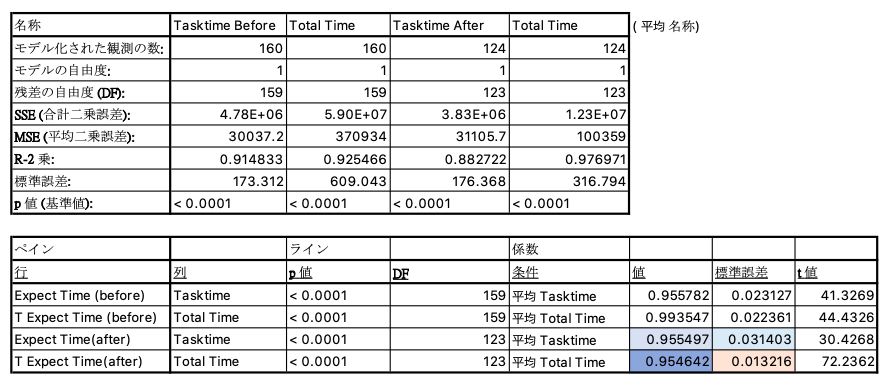
\includegraphics[width=15cm]{images/7/7.png}}
		\caption{ADLog導入前後の係数の比較(総合)}
		\label{fig:7}
	\end{center}
\end{figure}

また被験者の内訳に関しては表~\ref{fig:8},表~\ref{fig:9}に表した.
表~\ref{fig:9}では係数が高くなった被験者がいるものの,係数が下振れした被験者の方が多かった.

\begin{figure}[hb]
	\begin{center}
	\fbox{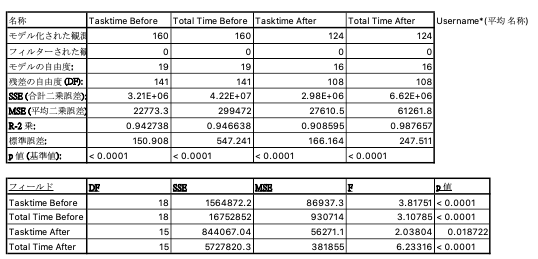
\includegraphics[width=15cm]{images/7/8.png}}
		\caption{ADLog導入前後の係数の比較(ユーザ別1)}
		\label{fig:8}
	\end{center}
\end{figure}
\begin{figure}[hb]
	\begin{center}
	\fbox{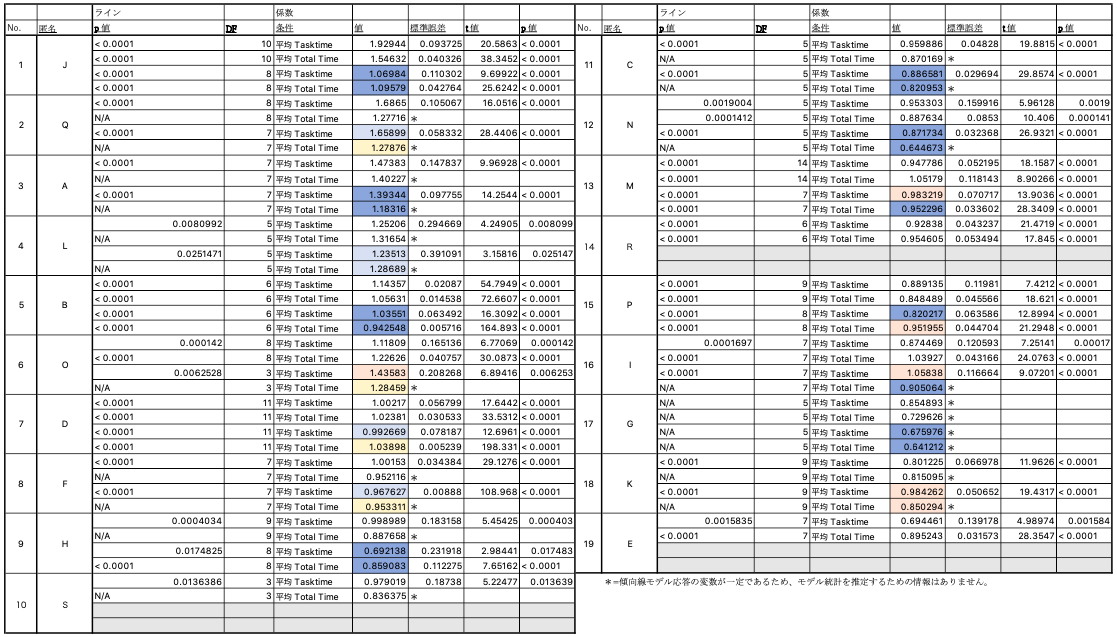
\includegraphics[width=15cm]{images/7/9.png}}
		\caption{ADLog導入前後の係数の比較(ユーザ別2)}
		\label{fig:9}
	\end{center}
\end{figure}

また係数比較だけではなく,箱髭図から分布を表~\ref{fig:9}にて表した.
表~\ref{fig:9}はタスク時間の秒数での分布,\%での分布,総合時間の秒数での分布,\%での分布を表しており,それぞれADLog導入前後の比較が出来る.
全ての分布はADLog導入後の方が分布が狭まり,総合時間に関しては中央値の値がやや高くなった事が分かる.
尚,ADLog導入後に見積もりの時間を変更したのは3人である.

\begin{figure}[hb]
	\begin{center}
	\fbox{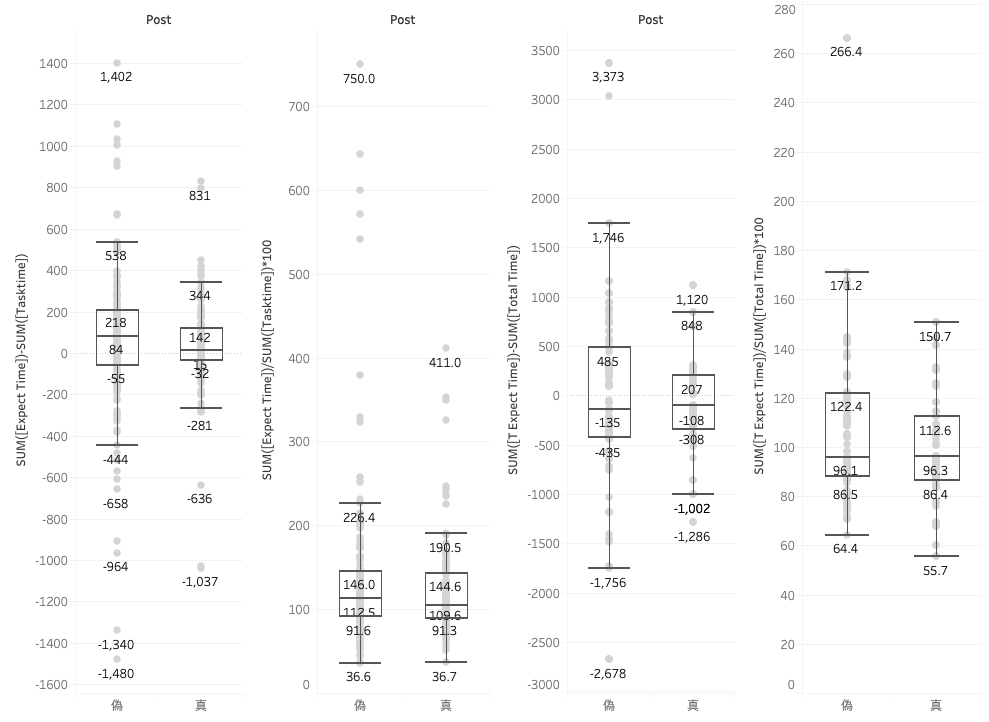
\includegraphics[width=15cm]{images/7/10.png}}
		\caption{ADLog導入前後の比較(箱髭図)}
		\label{fig:10}
	\end{center}
\end{figure}

また,被験者別の使用前後の比較を行ったところ図~\ref{fig:11},\ref{fig:12},\ref{fig:13},\ref{fig:14}の様になった.

\begin{figure}[hb]
	\begin{center}
	\fbox{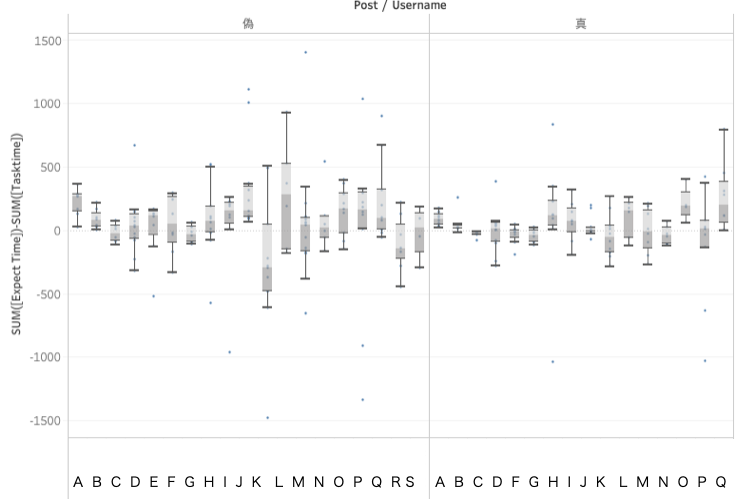
\includegraphics[width=15cm]{images/7/11.png}}
		\caption{ADLog導入前後の比較(タスク時間(秒))}
		\label{fig:11}
	\end{center}
\end{figure}

\begin{figure}[hb]
	\begin{center}
	\fbox{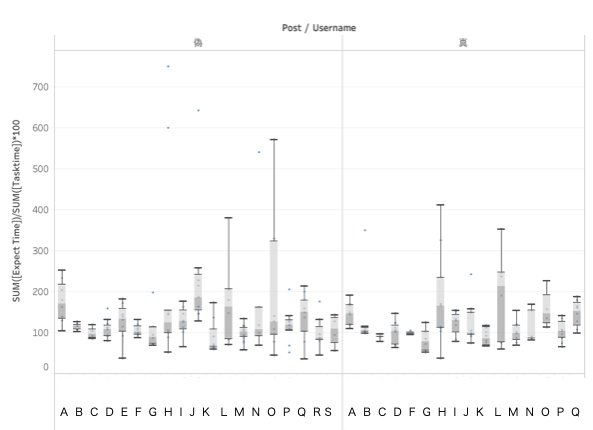
\includegraphics[width=15cm]{images/7/12.png}}
		\caption{ADLog導入前後の比較(タスク時間(\%))}
		\label{fig:12}
	\end{center}
\end{figure}

\begin{figure}[hb]
	\begin{center}
	\fbox{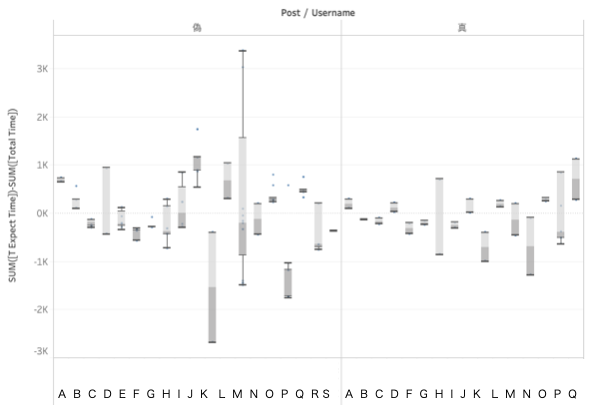
\includegraphics[width=15cm]{images/7/13.png}}
		\caption{ADLog導入前後の比較(総合時間(秒))}
		\label{fig:13}
	\end{center}
\end{figure}

\begin{figure}[hb]
	\begin{center}
	\fbox{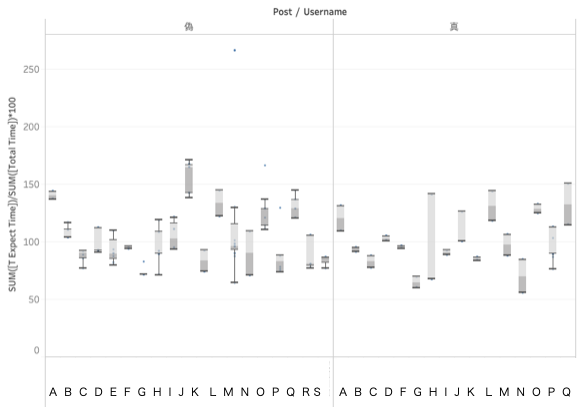
\includegraphics[width=15cm]{images/7/14.png}}
		\caption{ADLog導入前後の比較(総合時間(\%))}
		\label{fig:14}
	\end{center}
\end{figure}


\subsection{インタビューについて}
私は見積もり傾向と図の効果の有無から被験者を下記の様に分け,インタビューの質問項目など違いを調査した.
結果,まず苦手意識に関してはグループ\UTF{2460}の方が苦手意識を感じている被験者が少なく,\UTF{2461}・\UTF{2462}の被験者に苦手意識を感じている被験者が多かった.
また,見積もりを意図的に長く申告し少しゆとりを持たせている被験者はグループ\UTF{2460}・\UTF{2461}の被験者が多く,逆に\UTF{2462}に時間にゆとりを持たせて申告している被験者はいなかった.
更に,グループ\UTF{2460}(4/6人)と\UTF{2462}(4/7人)は\UTF{2461}(2/6人)と比較し,普段の生活では会話以外の作業(動画を見る,課題を行うなど)を行いながら朝の支度を行う場合が多いと回答した.
加えて,グループ\UTF{2460}(3/6人)と\UTF{2462}(2/7人)以外の11人に関しては平日(またはそれに準ずる日)と休日(〃)タスクの時間及びタスク間の時間に何らかの差があると述べた.

また,12人の被験者からはタイマー・予測時間の可視化によって安心感の向上や時間に対する効率化の意識の向上が発生したと述べていた.
\section{考察}
\subsection{アプリケーションの効果について}
実験結果から,ADLog機能導入によって見積もりの予測時間と実測時間の差が縮まる効果が得られた.特に時間管理に対し苦手意識のある被験者や見積もりの係数が1に近い被験者程効果が大きかった.
一方,ADLog導入後に見積もりの時間を変更した人はわずか3人である点,インタビューにて時間を意識すると述べている被験者が多かった事から本アプリケーションは
「見積もり傾向から自分の精度の悪い見積もりを修正する事によってズレが少なくなる」のではなく.「時間傾向の可視化に対しタイマーのカウントアップによって時間をより合わせる」効果をより発揮していると考えられる.

また,傾向線で見ると下振れしている被験者が多い事から.本機能の用いたバッファの取り方では見積もりを少なく見積もる様になってしまう可能性があり.バッファや目標時間は本機能の提示では正しく導けない事が分かる.
これは被験者別に傾向のタイプ分けをせず,かつまだ前例の無い中での暫定的な見積もりの提示をしており.より最適化が求められると考えられる.

\subsection{タイプ分けについて}
見積もり係数で分けた3グループ毎にADLogの効果に差がある事から,朝の準備に対し時間を見積もり,行動するパターンも少なくとも3パターンはあると考えられる.ここでは見積り係数の3グループを元に傾向を述べる.

グループ\UTF{2460}の被験者は見積りの時間を意識的に長く見積もる傾向にあり,見積り方はタスク自体を多めに見積もる人とバッファとして追加で数分余裕を持たせる人がいる.多くは毎日同じルーティンを行っている.
グループ\UTF{2460}は時間が余ることは既に想定内であり実際に時間が余った時のみ追加でやる事なども合わせて考えた上で行動を行う.時にはながら行動も行い,ゆとりがある事を前提として行動を見積もる.時間管理に対して苦手意識は感じない人が多い.

グループ\UTF{2461}の被験者は見積りの時間を実測値と丁度同じくらいに見積もる傾向にあり,本人の見積り方はバッファが存在する人としない人がいる.
多くはながら行動はあまり行わず,オンオフなどをはじめとして日によって朝行う行動も大きく変容する.
そのため毎日が均質なルーティンとして確立しておらず,日に合わせてその都度やることを意識下・無意識下関わらず組み立てた上で行動を行っており,時間管理に対し苦手意識を感じる被験者が特に多い.

グループ\UTF{2462}の被験者は大抵は実測値の方が見積もりより長くかかる傾向にあり,被験者のほとんどはバッファなどは存在しない為時間ぴったりを狙う人が多い.
グループ\UTF{2461}ほどでは無いがオンオフなどをはじめとして日によって朝行う行動も大きく変容し,時にはながら行動を行う.時間管理に対して苦手意識は感じない人と感じる人がいる.
尚,グループ\UTF{2462}で苦手意識の無い人はアプリの効果は薄かったと感じている人であり,実際の効果も同グループの苦手意識のある人に比べ薄かった.

グループ\UTF{2460}と\UTF{2462}に効果が出にくかった理由は,インタビューからもあまり効果が無いと述べる被験者も多かった事を踏まえると.
時間を基準に行動を行っていないのでは無く,自分の考える行動など別の基準により高い優先順位を置いている可能性が考えられる.
その為,苦手意識の無いグループ\UTF{2460}及び\UTF{2462}の被験者に対しては別のアプローチを用いて行動変容を試みた方が良いと考えられる.
\subsection{本評価実験での限界}
本実験はデータ数・被験者数が少ない事,短期間である事,一人一人のタスク行動が同一ではない事,時間の見積もり自体は個人間でも均一になりにくい事からデータの偏りが考えられる為更なる収集が必要である.
加えて本実験では被験日には実験者とzoomで話すというプロセスが組み込まれている事,実験は短期間である事からアプリケーションの効果をこの実験だけで評価することは厳しいと考えられる.

更に評価に関しても見積もりの予測傾向に関する理想のモデルは線形とは限らない.今後被験者同士を比較する評価を行う際には最適な傾向モデルを模索していく必要がある.
また,ずれの評価に関しては見積もりの失敗だけでなく複合的な原因が存在する可能性がある為,今後は本評価手法に限定せずに更なる評価実験が必要になると考えられる.
最後にアンケートにおいてはインタビューによる可能性の示唆を元に今後アンケートなどより統計的に評価しなおす意義があると考える.

\section{まとめ}
本章では,評価実験にの概要及び手法についてまとめたた上で,結果・考察を述べた.
次章では,本研究における今後の展望と本論文のまとめを述べる.
